\documentclass[answers]{exam}

% ------------------------------------------------------------------------------ %
% -----------------------      Base for every .tex file   ---------------------- %
% ------------------------------------------------------------------------------ %

\usepackage[dvipsnames]{xcolor}
\usepackage{mathtools}
\usepackage{amssymb}
\usepackage{amsthm}
\usepackage{amsmath}
\usepackage{framed}
\usepackage{wasysym}
\usepackage{geometry}
\usepackage{cancel}
\usepackage{blindtext}
\usepackage{pgfplots}
\usepackage{graphicx}
\usepackage{lastpage}
\usepackage[most]{tcolorbox} 
\usepackage{multicol}
\usepackage{soul}
\usepackage{listings}
\usepackage{algorithm}
\usepackage{algorithmic}
\usepackage{booktabs}
\usepackage{tikz}
\usepackage{pifont}

% Libraries
\usetikzlibrary{shapes,shapes.geometric, positioning, arrows}

\geometry{%
	left=15mm,
	right=15mm,
	top=25mm,
	bottom=25mm,
	bindingoffset=0mm,
	headheight=30pt,% output from geometry tells you what this needs to be set to as a minimum
}

% Header and Footer
\pagestyle{headandfoot}
\firstpageheadrule
\runningheadrule
\firstpageheader{Convex Optimization}{\today}{Jonathan Schnell}
\runningheader{Convex Optimization}{}{Jonathan Schnell}
\firstpagefooter{}{Page \thepage\ of \numpages}{}
\runningfooter{}{Page \thepage\ of \numpages}{}

% Commands
\newcommand{\imp}[1]{\ul{\textbf{#1}}}
\newcommand{\dproduct}[1]{\left\langle #1 \right\rangle}
\newcommand{\norm}[1]{\left\lVert #1 \right\rVert}
\renewcommand{\vector}[1]{\begin{pmatrix} #1 \end{pmatrix}}
\newcommand{\abs}[1]{\left| #1 \right|}
\newcommand{\floor}[1]{\lfloor #1 \rfloor}
\newcommand{\ceil}[1]{\lceil #1 \rceil}
\newcommand{\fracpart}[2]{\frac{\partial #1}{\partial #2}}
\newcommand{\set}[2]{\left\{#1 \ \middle|\ #2\right\}}
\renewcommand{\hat}[1]{\widehat{#1}}

\newcommand{\Ker}{\operatorname{Ker}}
\renewcommand{\Im}{\operatorname{Im}}
\renewcommand{\Re}{\operatorname{Re}}
\renewcommand{\dim}{\operatorname{dim}}
\renewcommand{\div}{\operatorname{div}}
\newcommand{\rot}{\operatorname{rot}}
\newcommand{\grad}{\operatorname{grad}}
\newcommand{\vol}{\operatorname{vol}}
\newcommand{\supp}{\operatorname{supp}}
\renewcommand{\div}{\operatorname{div}}
\newcommand*{\vertbar}{\rule[-1ex]{0.5pt}{2.5ex}}
\newcommand*{\horzbar}{\rule[.5ex]{2.5ex}{0.5pt}}

\theoremstyle{definition}
\newtheorem*{definition}{Definition}
\newtheorem*{beispiel}{Beispiel}
\newtheorem*{remark}{Remark}

\theoremstyle{plain}
\newtheorem*{proposition}{Proposition}
\newtheorem*{satz}{Satz}
\newtheorem*{korollar}{Korollar}
\newtheorem*{lemma}{Lemma}
\newtheorem*{theorem}{Theorem}


% Quote
\newtcolorbox{zitat}[1]{%
	colback=lightGray,
	grow to right by=-10mm,
	grow to left by=-10mm, 
	boxrule=0pt,
	boxsep=0pt,
	breakable,
	enhanced jigsaw,
	borderline west={4pt}{0pt}{gray},
	#1
}

% Use colors in equations
\newcommand{\highlight}[2]{\colorbox{#1}{$#2$}}%
\definecolor{lightGray}{gray}{0.9} 

% To add shortcut of script Letters in Equations
\newcommand{\s}[1]{\mathcal{#1}}
\newcommand*\circled[1]{\tikz[baseline=(char.base)]{
            \node[shape=circle,draw,inner sep=2pt] (char) {#1};}}
\newcommand{\cmark}{\ding{51}}
\newcommand{\xmark}{\ding{55}}


\newenvironment{claim}[1]{
		\par\noindent
		\textbf{Claim.} #1
		\begin{tcolorbox}[blanker, top=3mm, bottom=3mm, left=3mm, borderline west={1pt}{0mm}{black}]
		\noindent\textit{Proof of Claim.} 
}{
	\hfill$\blacksquare$	
	\end{tcolorbox}\noindent
}

% To add shortcut of number's set Z
\newcommand*{\Z}{\mathbb{Z}}
\newcommand*{\N}{\mathbb{N}}
\newcommand*{\R}{\mathbb{R}}
\newcommand*{\Q}{\mathbb{Q}}
\newcommand*{\C}{\mathbb{C}}
\newcommand*{\F}{\mathbb{F}}
\newcommand*{\K}{\mathbb{K}}

% To add shortcut of empty set
\renewcommand*{\o}{\varnothing}
\pgfplotsset{compat=1.9}

\everymath{\displaystyle}

% Line-Height
\linespread{1.15}

\graphicspath{{Files/}}

% ------------------------------

\begin{document}

	$ $
	\begin{center}
		\huge \textbf{Exercise session notes - Week 8}  \\ \vspace*{3mm}
        \Large{Gradient Descent + Types of Convexity in Descent Methods}
	\end{center}
	$ $\\

    \noindent This week we started with the new chapter on unconstrained Optimization. The goal is to solve the following unconstrained problem
    $$ \min\quad  f(x) \quad\text{for } x\in \operatorname{dom}(f)\subseteq \R^n $$
    The only requirement is that the function $f$ is twice differentiable.\\
    We first note that this problem can be sometimes solved analytically: we find a point $x^*$ with $\nabla f(x^*) = 0$, by solving a system of $n$ equations. This implies that the point $x^*$ is a local optimal solution, and if the function is convex, then $x^*$ is also a global optimal solution. Often this method cannot be applied as it is much slow, for example if $f$ does not have a closed form.

    In such cases we apply the Descent Method: we produce a sequence of points $x_0, x_1, x_2, \ldots$ with 
    $$ f(x_{j+1}) < f(x_j)\ ,\ f(x_j) \to f^* $$
    We have to answer two main questions: Given a point $x_0$
    \begin{itemize}
        \item In which direction we move to get $x_1$? (Step Direction)\\
        In class we saw the Gradient descent, which uses $\Delta x = -\nabla f(x)$.
        \item How much we have to move in direction $\Delta x$? (Step Size)
        \begin{itemize}
            \item Exact Line Search: we find the optimal step size in direction $\Delta x$
            \begin{center}
                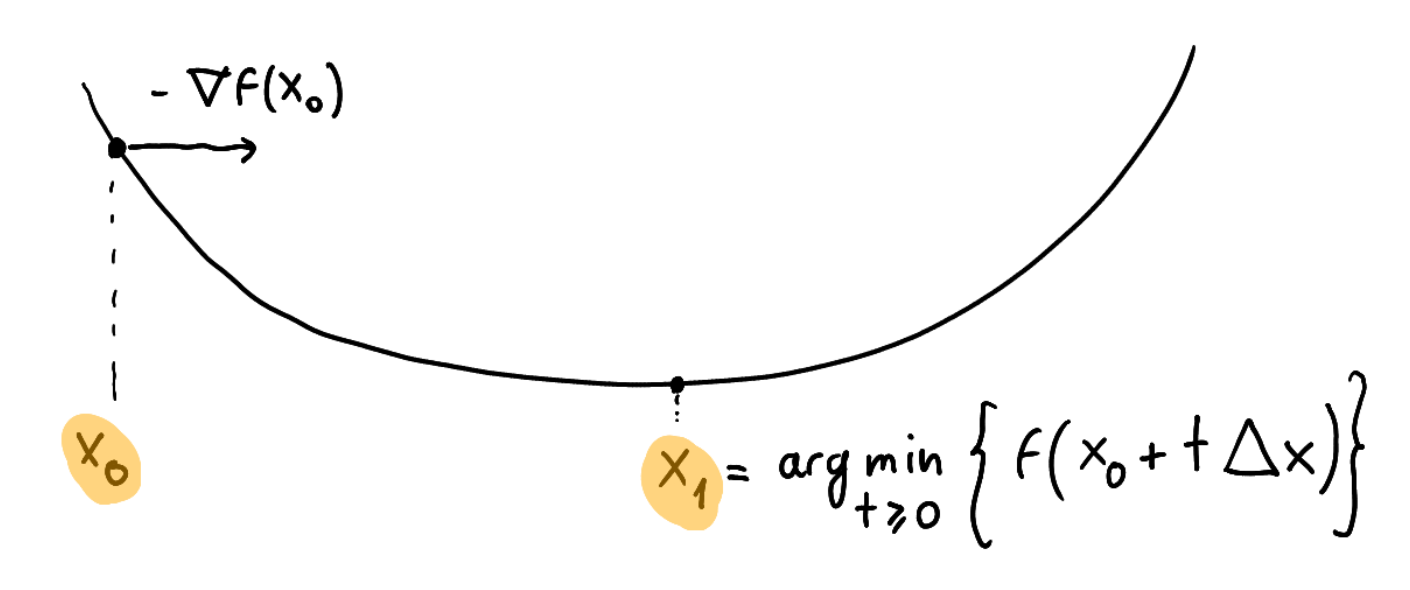
\includegraphics[width=0.5\textwidth]{ExactLineSearch.png}
            \end{center}
            \item Backtracking Line Search: we move one unit in direction $\Delta x$ and then backtrack until we meet some requirements 
            \begin{center}
                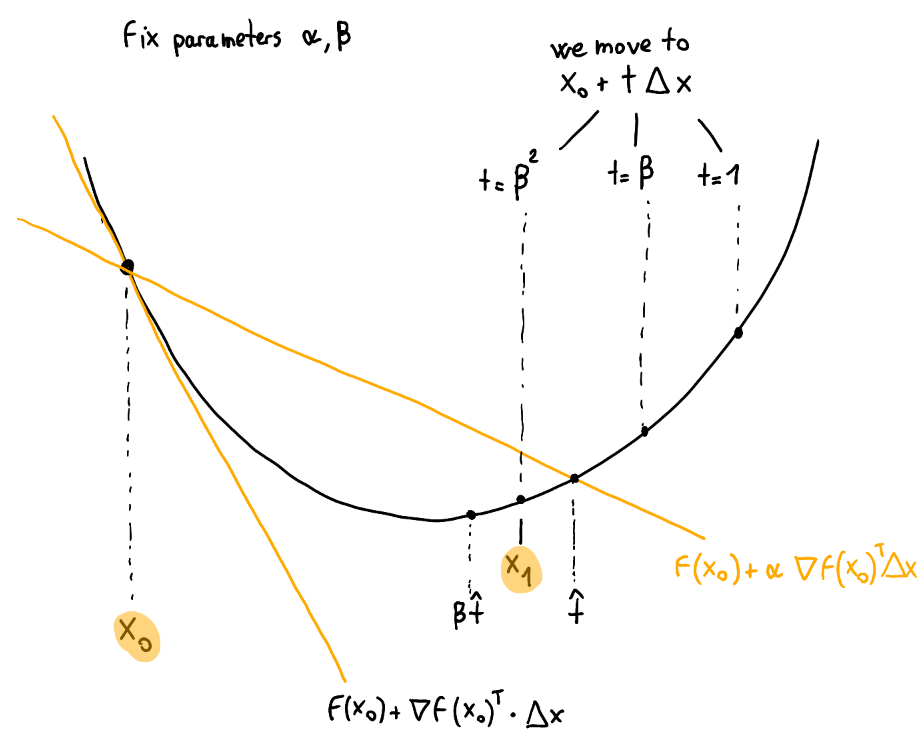
\includegraphics[width=0.5\textwidth]{BacktrackingLineSearch.png}
            \end{center}
        \end{itemize}
    \end{itemize}
    Finally we reviewed the different types of convexity:
    \begin{itemize}
        \item If $f$ is not convex, then the Descent Method (usually) finds a local optimum; this is often the case in machine learning.
        \item If $f$ is convex, then the Descent Method (usually) finds a global optimum, but not always (consider the convex function $-\log(x)$).
        \item If $f$ is strictly convex, then the Descent Method (usually) finds a global optimum. This usually does not give us any additional properties compared to the convex case (consider the strictly convex function $e^{-x}$)
        \item If $f$ is stongly convex, then the Descent Method always finds a global optimum in a finite amount of time. This is the property that we usually look for.
    \end{itemize}
    We concluded the ex. class an important proposition on strong convexity that is a good practice exercise.
    \paragraph{Proposition.} If $f$ is strongly convex with constant $m > 0$, then it is also coercive, i.e.
    $$ \lim_{\norm{x} \to \infty} f(x) = \infty $$
    In particular, there always \underline{exists} an \underline{unique} global minimum. 
\end{document}